% Overview of section
In the previous section, we described how \code{rfactor} transforms a Halide reduction to expose new data parallelism. Doing so requires synthezising the associative binary operator equivalent to the Halide \emph{update} definition being factored. In this section we describe how we do this synthesis.

% Set up problem, LUT solution
In some cases generating the equivalent associative operator from an update definition is trivial (e.g.\ summation). In other cases it is not, especially when the function reduces onto multiple values (see the examples in Figure~\ref{fig:subgraphs}). The \emph{inverse} problem is easier: Given an associative binary operator, it is straightforward to generate the Halide update definition that implements reduction by it. Therefore, if there were a \emph{small} finite set of associative binary operators, we could simply attempt to match the update definition being factored against each of them in turn. Halide already includes facilities for doing regex-like matching of expressions against patterns with wildcards. Unfortunately, there are more meaningful associative binary operators than could reasonably be thought of ahead of time by a compiler author.

% Full synthesis solution
An alternative approach is to use program synthesis techniques~\cite{Solar-Lezama:2008:PSS:1714168, Torlak:2013:GSL:2509578.2509586} to synthesize the corresponding associative reduction at compile-time when the call to \code{rfactor} is made. This is intractably slow, and can increase compile times of Halide pipelines from seconds to hours.

% Our solution
We use a hybrid of the two approaches, amplified with a strategy for decomposing each synthesis problem into several simpler problems. Offline, we generate a \emph{large} finite table of one- and two-dimensional \emph{elementary} associative binary operators and their identities. These are akin to primes -- they are the associative operators which cannot be decomposed into a combination of simpler associative binary operators. At compile-time, we decompose the given Halide update definition into a composition of simpler, lower-dimensional definitions in the same way, then search the table for the elementary operator corresponding to each. If consistent matches are found, we reassemble the results into a composite associative operator equivalent to the original update definition. In Section~\ref{subsec:generation} we describe how we generate the table, and in Section~\ref{subsec:decomposition} we describe the decomposition procedure.

\subsection{Generating Elementary Operators}
\label{subsec:generation}

We begin with an enumeration of all one- and two-dimensional tuples of expression trees in two inputs $x$ and $y$. $x$ and $y$ are themselves tuples. The operators used to form the inner nodes of the trees are Halide's IR nodes (\code{*}, \code{+}, \code{-}, \code{min}, \code{max}, \code{select}, \code{<}, etc). We can reject some classes of uninteresting expressions by excluding them from the enumeration altogether. We only generate trees which use both $x$ and $y$. For every commutative operator in the tree, we only generate subtrees where there are at least as many leaves on the left as the right (TODO: how do we account for this during matching? and why this restriction?). We generate trees using a single generic constant $k$, rather than generating trees containing all possible constants as leaves. We do not generate trees that would be trivially simplified (For example, we do not generate subexpressions like $max(x_0, x_0)$).

We then subject the expressions to a battery of tests so that only elementary associative operators remain. The tests are arranged in increasing order of expense, so that we can cheaply reject most expressions.

\begin{enumerate}
\item We first apply both the Halide simplifier and solver to the expression, which simplifies and canonicalizes it in certain ways (e.g. in a tree of commutative operations, $x_i$ is always to the left of $x_{i+1}$ if possible, and constants are always on the right). All inputs to the matching process will have gone through the same process, so if the expression was mutated by the simplifier or solver, then we will never expect see it as an input and so it can be discarded.
\item For an operator $f$, we construct the expressions $f(f(x, y), z)$ and $f(x, f(y, z))$, and substitute in 100 randomly-selected values for $x, y, z$. If the two expressions don't evaluate to the same thing, the expression is not associative and can be rejected.
\item We then reject operators which can be decomposed using the decomposition procedure in Subsection~\ref{subsec:decomposition}.
\item Finally, to \emph{prove} that the expression is associative, we ask Z3~\cite{DeMoura:2008:ZES:1792734.1792766} to verify that $\forall x, y, z, k \;f(f(x, y), z) = f(x, f(y, z))$. If this proof succeeds, we ask Z3 to solve $\forall x, k \;f(id, x) = x$ to synthesize the identity $id$.
\end{enumerate}

In the table of expressions that this produces, $x$ represents the partial result being reduced onto, and $y$ is a wildcard which could match any expression. When matching, $x$ must also appear on the left-hand-side of the update definition. $y$ may depend on the reduction domain coordinates, but may not depend on the partial results. The constant $k$, if it exists, may match anything which neither depends on the reduction domain coordinates nor the partial result. For example, the update definition which separately computes the sum-of-squares of the even and odd values of some input \code{in} could be written as:

\code{f(in(r) \% 2) = f(in(r) \% 2) + pow(in(r), 2)}

This would match against the pattern $x + y$, where $x$ matches \code{f(in(r) \% 2)}, and $y$ matches \code{pow(in(r), 2)}.

We terminate our enumeration at trees with 8 leaves. We generate separate tables for each of Halide's scalar types, as some operations are associative in one type by not another. This takes TODO hours and generates TODO elementary operators to match against. The first 10 elementary associative operators for signed 32-bit integers are shown in Listing~\ref{lst:top10}.

\begin{lstlisting}[caption={The first 10 elementary associative operators for 32-bit signed integers}, label={lst:top10}]
x + y
x * y
min(x, y)
max(x, y)
max(min(x, k), y)
min(max(x, k), y)
max(min(y, k), x)
min(max(y, k), x)
max(min(k - x, y), x)
min(max(k - x, y), x)
\end{lstlisting}

As we only consider one- and two-dimensional expressions, there are meaningful primitive operators that we never discover. For example, we never generate quaternion multiplication. It is an elementary associative operator in 4 tuple elements, where every expression tree has 8 leaf nodes. We must add any important higher-dimensional primitive operators to our table manually. Another limitation is that for each associative reduction, we have a single pattern for the update definition we expect to see, and so if the Halide simplifier and solver fail to canonicalize an update definition into that form, we will not recognize it. For example, consider the reduction which counts how many points in the reduction domain satisfy some predicate $P$. If the programmer writes it with the addition outermost, e.g. as \code{f() = select(P(r), 1, 0) + f()}, then after canonicalization we recognize it as a sum reduction of the form \code{x = x + y}. If the programmer writes it with the \code{select} outermost as \code{f() = select(P(r), f() + 1, f())}, then we do not recognize it as a sum reduction.

\subsection{Subgraph Decomposition}
\label{subsec:decomposition}

To talk about how we decompose reductions into elementary operators, we must first discuss how one might \emph{compose} elementary reductions. The simplest way to compose two reductions into a higher-dimensional reduction is to compute them both of them at the same time independently. This means that reductions that are a concatenation of smaller independent associative reductions are also associative. For example:

\code{f() = \{f()[0] + in(r), f()[1] * in(r)\}}

is associative, because it is a composition of the following two associative reductions:

\code{f0() = f0() + in(r)}

\code{f1() = f1() * in(r)}

Secondly, if we have an associative operator in which two tuple components compute the same value, we can deduplicate it, reducing the dimensionality by one. The result is still associative. Therefore, we can prove a reduction is associative by duplicating one of the elements to break a dependency and then applying the rule above. Consider the case of two-dimensional argmin:

\begin{lstlisting}[caption={Two-dimensional argmin. The three tuple components are the minimum value, and its x and y coordinates.}]
f() = {min(f()[0], in(r.x, r.y)),
       select(f()[0] < in(r.x, r.y), f()[1], r.x),
       select(f()[0] < in(r.x, r.y), f()[2], r.y)}
\end{lstlisting}

All three tuple components depend on \code{f()[0]}, so we can't decompose this into independent reductions immediately. Let's duplicate the first tuple component to break the dependency:

\begin{lstlisting}[caption={Two-dimensional argmin with the minimum value redundantly computed as \code{f()[0]} and \code{f()[2]}}]
f() = {min(f()[0], in(r.x, r.y)),
       select(f()[0] < in(r.x, r.y), f()[1], r.x),
       min(f()[2], in(r.x, r.y)),
       select(f()[2] < in(r.x, r.y), f()[3], r.y)}
\end{lstlisting}

There are no dependencies between the first two components and the last two. This is now a simple concatenation of two single-variable argmin operations. Single-variable argmin uses two tuple components, and is present in our table of primitive oeprators, so we regonize two-dimensional argmin as associative via its decomposition into two one-dimensional argmin reductions.

In general we consider the directed graph of dependencies between tuple elements. There is a vertex per tuple element, and an edge from vertex $i$ to vertex $j$ whenever the definition of tuple element $i$ refers to tuple element $j$. If we repeatedly duplicate vertices (tuple elements) to break dependencies, in the limit, the graph has one connected component per original tuple element, and that component is the subgraph containing the vertices reachable from that tuple component. If each such subgraph is an associative reduction, then the original reduction is associative. See Figure~\ref{fig:subgraphs} for several examples.

%The general way to apply these two rules to decompose an arbitrary reduction into its components is to construct the directed graph $G$ of dependencies between tuple components. There is a vertex $N_i$ for each tuple component $i$, and there is an edge from $N_i$ to $N_j$ whenever the value of tuple component $i$ depends on tuple component $j$. The two rules above can then be stated as:

%\begin{enumerate}
%\item If every connected component of $G$ is an associative reduction, then $G$ is an associative reduction.
%\item If we duplicate one of the nodes of $G$, partitioning its incoming edges arbitrarily between the two copies, then the resulting graph is associative iff $G$ is associative, as they compute the same thing.
%\end{enumerate}

% This is a shitty ``proof''
%Let the subgraph $S_i$ be all vertices and edges reachable from $N_i$. We can make a copy of $S_i$ as its own connnected component set apart from the rest of $G$ by the following procedure: Initialize $S_i$ to contain only a duplicate of $N_i$, with no incoming edges. Then repeatedly consider all edges that leave $S_i$, and make duplicates of the vertices they point to, where edges from vertices within $S_i$ point to the duplicate, and edges from vertices not in $S_i$ point to the original. This procedure terminates when $S_i$ contains all vertices reachable from $N_i$. At that point, there are no edges between $S_i$ and the rest of $G$, so it is its own connected component. Once we construct each such $S_i$, we can discard $G$, as everything it computes is also computed by one of the disconnected subgraphs. Similarly, we can discard subgraphs which are completely contained by some other subgraph. Therefore, if every subgraph $S_i$ not contained within some other subgraph is an associative reduction, then $G$ is an associative reduction. For examples of these graphs and their subgraphs for several reductions see Figure \ref{fig:subgraph}.

\begin{figure}
\centering
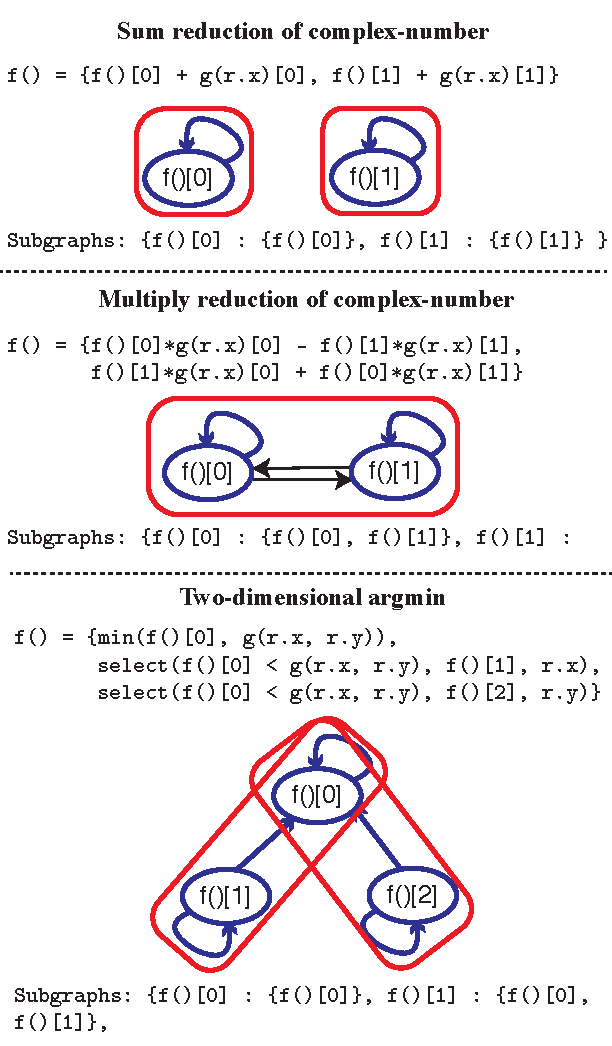
\includegraphics[width=3.2in]{subgraphs}
\caption{Dependency graphs of various multi-valued Halide \emph{update} definitions. Their subgraph decompositions are shown in red. To find the associative operator equivalent to a complex Halide update definition, we first decompose it into subgraphs, then search for each subgraph in our precomputed table of elementary operators, then recompose the results into a single multi-valued associative operator.}
\label{fig:subgraphs}
\end{figure}

% Merging results of decomposition
After finding the associative operator equivalent to each subgraph separately, we need to combine the results into a single associative operator equivalent to the entire update definition. If any of the subgraphs are non-associative (or we fail to find the equivalent binary associative operator or an identity), we terminate and return an error. If a single tuple element appears in multiple subgraphs, we need to ensure that the binary associative operators deduced via each subgraph are all the same in that tuple element. If there is contradiction, we terminate and return an error. In the cases where the reduction is indeed associative, but we have failed to prove that fact and have thus refused to apply \code{rfactor}, the programmer must manually factor the reduction.

\begin{figure}
\centering
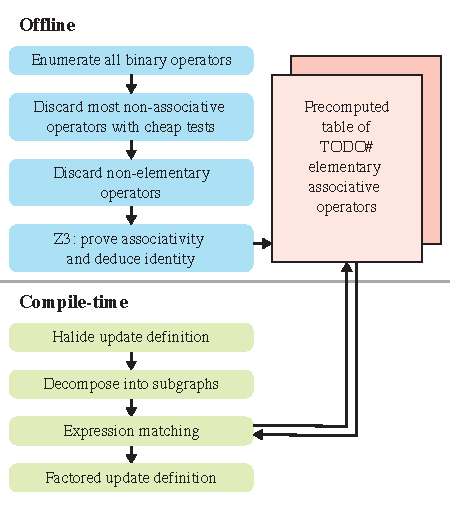
\includegraphics[width=3.2in]{system}
\caption{To factor a reduction written as a Halide update definition, we must first synthesize the equivalent associative binary operator. We generate a large table of elementary associative operators offline by enumerating all non-trivial expression trees and filtering out the ones that are not associative operators. At compile-time, we then decompose the given update definition into simpler definitions and match each against the table. Combining the results gives us the equivalent associative binary operator, which we can use to generate the factored form of the reduction}
\label{fig:system}
\end{figure}
